\documentclass[12pt,a4paper]{scrartcl}		% KOMA-Klassen benutzen!

%\usepackage[ngerman]{babel}			% deutsche Namen/Umlaute
\usepackage[utf8]{inputenc}			% Zeichensatzkodierung
\usepackage{url}
\usepackage{graphicx}
\usepackage[colorlinks=false, pdfborder={0 0 0}]{hyperref}
\usepackage{amsmath}

\usepackage{setspace} % Anderthalbfacher Zeilenabstand ist Standard in den meisten Seminararbeiten. Das Paket setspace ermöglicht ein einfaches Umstellen von normalem, anderthalbfachen oder sogar doppeltem Zeilenabstand. 
\usepackage[paper=a4paper,inner=25mm,outer=20mm,top=15mm,bottom=20mm]{geometry} %Das geometry Paket dient zur Einrichtung der Seiten. Hier werden die jeweiligen Seitenränder angegeben. Diese wWerte sollten durch die jeweiligen Vorgaben des Seminarleiters oder Instituts ersetzt werden.
\setlength{\parindent}{1.7em} %Neue Abschnitte werden mit hängendem Einzug gesetzt, parindent definiert. um wie viel der Absat eingerückt wird. Die Einheit em ist abhängig vom verwendeten Zeichensatz und daher absoluten Werten in mm oder cm vorzuziehen. 
\setcounter{secnumdepth}{3} %Bis zu welcher Gliederungsebene nummeriert werden soll gibt dieser Befehl vor. In diesem Falle werden \section, \subsection und \subsubsection nummereiert.
\setcounter{tocdepth}{3} %Bis zu welcher Ebene Einträge ins Inhaltsverzeichnis aufgenommen werden. In diesem Beispiel ebenfalls bis Ebene drei (\subsubsection). Ein durch \paragraph ausgewiesener Abschnitt wird demnach nicht im Inhaltsverzeichnis auftauchen. 


\begin{document}
\title{HadoopDB}
\subtitle{a major step towards a dead end}
\author{Thomas Koch}
\date{\today}
\maketitle{}

\begin{abstract}
  
\end{abstract}
\tableofcontents{}

\section{NoSQL and the end of an architectural era}
In 2007 a paper with the provoking title ``The end of an architectural era:(it's time for a complete rewrite)''\cite{sto07} claimed that the time for traditional relational database management systems would be over. Current RDBMSs have their roots in nearly thirty years old legacy code lines. They are build on assumptions, requirements and hardware constraints that no longer hold true today and should therefor be replaced by a collection of specialized engines.

The change in Hardware is the most obvious. Main memory (RAM) on servers, CPU speed, number of CPUs and storage size have all increased by several orders of magnitude while at the same time hardware price decreased. In former times it was feasible to pay high salaries for specialized staff to administrate and optimize hardware. Today it is a decent decision to buy more hardware and spare costly developer time.

At the time systems like SQL Server, DB2 or Oracle were architected, they targeted the only then existing database market which back then was business data processing. Today several new markets exists:

\begin{itemize}
\item Text (search engines, translations)
\item Data Warehouses
\item Stream Processing (social networks, news sites, real time communication)
\item Scientific and intelligence databases (semantic data)
\end{itemize}

For all this use cases, specialized systems can outperform RDBMSs by a factor of 10.\cite{conf/cidr/StonebrakerBCCGHHLRZ07}. Stonebrakers findings and conclusions correspond with the views of many proponents of the so called ``NoSQL'' movement. His text from 2007 has therefor been proposed as an introductory reading for an international nosqlsummer in 2010.\footnote{\url{http://nosqlsummer.org/papers} The author was the organizer of the nosqlsummer meetings at lake Constance.} 

Although Stonebraker and his co authors (one of them is Daniel J. Abadi, the main author of the HadoopDB paper) make a strong point against RDBMSs and for alternative systems, the next section will discuss how they oppose MapReduce in favor of parallel databases and by doing so ignore their own arguments made against relational systems.

\section{The MapReduce vs. parallel databases debate}
In an online article from January 2008, published on the website of the database company Vertica Systems\footnote
{According to Wikipedia Stonebraker is co-founder of Vertica Systems, which has recently (march 2011) been acquired by HP. Footnote 9 in \cite{journals/pvldb/AbouzeidBARS09} discloses that also Daniel Abadi has a small financial stake in the company.},
Stonebraker heavily criticizes MapReduce.\cite{sto08stepback} The article has been commented (in comments on the same page or in blog posts\cite{Chu-Carrol08hammers}) as being inaccurate or missing the point. The main inaccuracy comes from judging MapReduce in areas which it has not been designed for especially judging it as a DBMS, which it isn't.

Since 2008 MapReduce and its supporting tools have made a lot of progress. Therefor it makes sense to revisit some of the arguments and consider recent developments.

\subsection{Understanding of the term MapReduce}
As Stonebraker rightly points out, MapReduce is not novel. In its core it's just the concept of using a map and a reduce function and in this a basic concept of functional programming. MapReduce can work on different underlying data stores: the Google File System (GFS), Hadoop Distributed File System (HDFS), databases like HBase and Cassandra. These are all systems for large data sets. But MapReduce is also a main building in CouchDB which uses views and B-Trees and targets server installations as well as mobile devices.

In the discussed papers the term MapReduce however is used to describe the combination of a scalable, fault tolerant file system (GFS or HDFS) together with a batch processing execution framework (Hadoop or Google MapReduce).
This inaccurate term usage may contribute to some of the misunderstandings discussed below. This text will however adapt to this nomenclature for the sake of readability.

\subsection{Rebuttal of MapReduce criticism}
\paragraph{Lack of schemes}
MapReduce has no support of schemes since it does not aim to be a database. However the object serialization projects avro, protocol buffers and thrift provide facilities to define schemes in one central place or together with the data and use them from most popular programming languages.\footnote{avro: \url{http://avro.apache.org/}, protocol buffers: \url{http://code.google.com/p/protobuf}, thrift: \url{http://thrift.apache.org}}

\paragraph{Lack of high level access languages}
Pig and Hive\footnote{Pig: \url{http://pig.apache.org}, Hive: \url{http://hive.apache.org}} lists their first releases on their websites as being from late 2008 or early 2009. Stonebraker also mentions them in 2009\cite[p. 3, sec. 3.3 programming model]{Pavlo09}. Around the same time Cascading\footnote{\url{http://www.cascading.org/}} appeared. But still in 2009 he fails to recognize that MapReduce should not be judged as a RDBMS but as a programming framework which is versatile enough to be also a foundation for some kind of database.

To make the list complete there are also Jagl from IBM and the not so active Cloudbase\footnote{Jagl: \url{http://code.google.com/p/jaql}, Cloudbase: \url{http://cloudbase.sourceforge.net}}. Unlike the systems mentioned so far Googles Sawzall\footnote{\url{http://code.google.com/p/szl}} while also being free software does not (yet) work with Hadoop.

Since MapReduce is not a database but a platform it is even possible to implementations applications on top of it which would be impossible to model with SQL like machine learning. The Mahout project\footnote{\url{http://mahout.apache.org}} is exactly that.\footnote{some pointers taken from: \url{http://www.hpts.ws/session10/shekita.txt}}

\paragraph{Missing features}
While it may not be fair to compare the tool set of decades of relational database development with those of the young MapReduce world, there is still already quite something to mention for the categories questioned:

\begin{itemize}
\item Bulk loader: Sqoop\footnote{\url{https://github.com/cloudera/sqoop}} is developed by Cloudera to transfer data between Hadoop, relational databases and other means. Besides that there are multiple projects to continuously import stream data into Hadoop: Flume, Scribe and Chukwa\footnote{\url{http://nosql.mypopescu.com/post/820711193/how-does-flume-and-scribe-compare}}.
\item Indexing: The Belgian CMS company Outerthought is pioneering to build its newest CMS on top of HBase and therefor also Hadoop. For its content repository it evaluated different scalable indexing solutions to provide secondary indexes into HBase.\footnote{\url{http://www.lilyproject.org/lily/about/technology.html}} Outerthought has been included by Gartner in "Cool Vendors in Content Management 2010" list.\footnote{\url{http://outerthought.org/blog/373-ot.html}}
\item Updates: MapReduce or better said the Google File System respectively HDFS have been developed for big files that are written once and never changed. On top of that Googles BigTable or Apache HBase provide databases for random access and updates to small data items.
\item Transactions: When Googles BigTable database was implemented, transactions were left out initially. Later on it was observed, that there was actually no real need to support them, because most applications require only row level isolation.\cite[p. 12]{Chang:2006:BDS:1267308.1267323} The developers of the web service streamy.com give a description how they started development with a normalized scheme on a RDBMS and had to denormalize there scheme step by step to scale the service. In the end they gave up on their RDBMS altogether and used HBase instead.\cite[p. 431-435]{White201010}
\item Integrity constraints: As with transactions one can argue that most use cases for MapReduce don't have the need for integrity constraints. Data that is handled by MapReduce is often collected from unreliable or unstructured sources like web pages, log files or sensors. It is desirable to also save corrupted data, like invalid HTML or out of scale measured data. This data can after wards be simply ignored by MapReduce jobs but is still available for further analysis. A search engine could for example reduce the ranking of domains with many invalid HTML pages or in a sensor network one could identify sensors which often produce erroneous values. So in the world of MapReduce integrity is handled at read time, not at write time. Different MapReduce jobs may have different opinions about which data they consider worth of further examination.
\item Referential integrity: See the argument on transactions. When the scheme is denormalized there is no need for referential integrity. Furthermore with data at scale one may need to give up on perfect data. Web links may point to nonexistent pages, Users may have deleted their accounts, changed their name or email address.
\item Views: I'm not aware of anything similar in MapReduce related technology nor have I ever read a complaint about its absence. But as we've seen above tools on top of MapReduce gets developed when needs for them occur.
\end{itemize}
As with the lack of features Stonebraker misses integration with DBMS tools. At least for Business Intelligence this may not be the case anymore since Pentaho announced Hadoop support in may 2010.\footnote{\url{http://www.pentaho.com/news/releases/20100519_pentaho_harnesses_apache_hadoop_to_deliver_big_data_analytics.php}}

\section{Discussion of MapReduce vs. parallel databases benchmarks}
The previous section discussed the misconception about MapReduce being a database. In line with this misconception Stonebraker, Abadi et al. moved on to directly compare performance between MapReduce and two RDBMSs.\cite{Pavlo09} This section discusses some of the flaws of this work.
The benchmarks were made on a cluster of at maximum 100 machines. This decision is justified by the ``superior efficiency of modern DBMSs'' that would not require more hardware to work on petabyte scale. This argument will be revisited in this section. Additionally the necessity for such large data sets is generally questioned:
\begin{quote}
  Since few data sets in the world even approach a petabyte in size, it is not at all clear how many MR users really need 1.000 nodes.
\end{quote}
This proposition sounds a lot like the famous (mis)quotes ``I think there is a world market for maybe five computers'' and ``640K ought to be enough for anybody''. While it may not be desirable from an energy efficiency or data privacy point of view to have many petabyte clusters, it only needs a little imagination to come up with many valid use cases. Millions of smart phones with cameras produce an immense amount of pictures and videos. Modern cars have sensors and computers build in whose data could (or is?) used to improve the next generation of cars. Science analyzes large data sets in genetics or high energy physics. The Global Biodiversity Information Facility is currently evaluating Hadoop.

\paragraph{Fault Tolerance}
The probability of one node failure in a cluster is a linear function of the number of cluster nodes which in turn depends on the data size:
\begin{equation*}
  p_{failure cluster} \sim p_{failure node} \cdot n_{nodes} \sim p_{failure node} \cdot datasize
\end{equation*}
In most cases the algorithms are at least $O(n log n)$. So with growing data size one can expect single node failures during the execution of a computation. A system that restarts the whole computation on a single node failure, as typical in RDBMSs, may never be able to complete on large enough data sizes.
By limiting the benchmark to a cluster of 100 nodes this problem is practically avoided. Abadi discusses and addresses the problem in the HadoopDB work.\cite{journals/pvldb/AbouzeidBARS09}.

\paragraph{Data Loading}
The discussed benchmarks all create a set up in which data is prepared and loaded into a data analytics cluster just for the purpose of the analysis. It is assumed that the data is imported from some other data store that is responsible for reliable long term storage and backup.
This however is not the typical use case of GFS or HDFS. These file systems are used to collect the raw incoming data from crawlers, sensors, log files or user actions. Instead of moving this data to a separate analytic cluster, MapReduce works directly on the original data, perhaps storing the computed data to a separate data store.
The validity of the given benchmarks is therefor highly questionable. A realistic benchmark would need to consider the necessity for reliable storage and parallel writes. A separate ``data loading phase'' however does not exist.

\paragraph{Problem Space}
One of the benchmarks, the ``Selection Task'' works on input that already combines a url with its page rank. This may server as an indicator for the complete misunderstanding of the different problem space of MapReduce opposed to that of RDBMSs. The original MapReduce paper explicitly names the ``Reverse Web-Link Graph'' as an example task for MapReduce. The output of this task is the input to calculate page rank. This algorithm is one of the model use cases for MapReduce.

The benchmark however assumes the page rank as a given input data for a task that is indeed a proper use case for a RDBMS and not for MapReduce. MapReduce users usually do not deny the usefulness of RDBMSs in their appropriate problem space. Facebook for example has been reported to use Oracle and MySQL to analyze data that has been prepared by Hadoop. (Figure~\ref{fig:facebookdatawarehouse})

\begin{figure}[t]
  \centering
  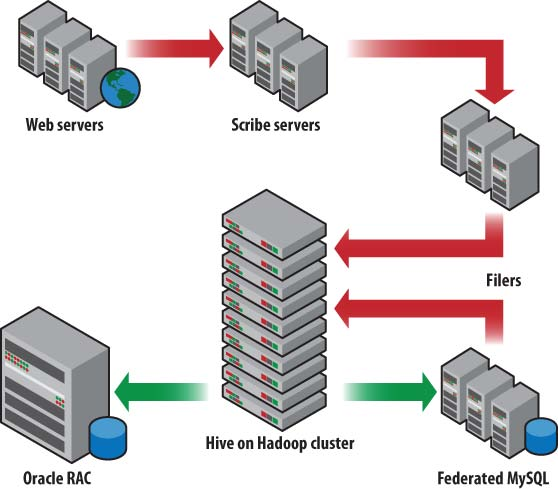
\includegraphics[width=0.7\textwidth]{images/rdms_as_frontend.jpg}
  \caption{Data warehouse architecture at Facebook\cite[p. 508]{White201010}}
  \label{fig:facebookdatawarehouse}
\end{figure}

There are more details to discuss in Stonebrakers benchmarks but this is left to a separate work. Other points are explored in the benchmarks of HadoopDB.

\section{HadoopDB}

\subsection{Motivation}

HadoopDB is a project to address the assumed shortcomings of MapReduce in analytical applications by using many single node RDBMSs as storage and local processing layer. However previous sections already concluded that MapReduce has different application areas compared to relational systems and that the assumed shortcomings of MapReduce are not valid but rather misunderstandings.

Since HadoopDB is based on such questionable ground it may be very well possible, that the project does not really address any real need and provides no practical usability. The current section discusses exactly that.

\paragraph{Desired Properties}
HadoopDB aims to provide the following list of properties. It is argued that neither MapReduce nor parallel databases succeed in these areas.

\begin{itemize}
\item Performance: It is claimed, that performance differences could ``make a big difference in the amount, quality, and depth of analysis a system can do''. Also performance could significantly reduce the cost of an analysis if fewer hardware ressources were used. However Stonebraker and Abadi concluded already in 2007 that the primary factor for costs has shifted from hardware to personal.\cite[2.5 No Knobs]{sto07} It should also be considered that the costs for licenses of proprietary database systems often outrun hardware costs by orders of magnitude. Finally it is not at all certain, that in practice performance differences are a limitation factor for the range of possible computations.

The paper suggests that current practice in analytical systems is to load data in a specialized database and to make calculations while an operator is waiting for the results. In MapReduce systems however calculations are directly done on the original data and could therefor run continuously during the normal operation of the system.
The authors own practical experience suggests that the limitation factor for data analysis is normally the time and competence of the personal in charge of preparing and interpreting the analysis.
\item Fault Tolerance: Abadi describes fault tolerance in the context of a read only analytical database. Hadoop however targets the requirement of concurrent read and write access with persistence guarantees and high availability. Fault tolerance can stand in direct conflict to performance. In this cases parallel databases tend to trade of fault tolerance in favor of performance while Hadoop is doing the opposite, e.g. by doing frequent checkpoints during MapReduce executions.
\item Ability to run in a heterogeneous environment: The system needs to make progress in the presence of individual node failures and its performance may not be bound by the slowest nodes.
\item Flexible query interface: The system should support SQL to integrate with existing tools as well. Ideally it also supports user defined functions (UDF) and manages their parallel execution.
\end{itemize}
The above list does not include energy efficiency as a desired property although it is one of the most important subjects in recent discussions about data centers.\footnote{see Googles Efficient Data Center Summit, 2009 \url{http://www.google.com/corporate/datacenter/summit.html} and Facebooks open compute project \url{http://opencompute.org}} It has also been argued, that standard performance benchmarks should be enhanced to measure the performance relative to the energy consumption.\cite{Fanara:2009:SEP:1692899.1692904}

\subsection{Architecture}
Hive is tool that provides a SQL interface to MapReduce. It translates SQL queries into apropriate combinations of map and reduce jobs and runs those over tabular data stored in HDFS. HadoopDB extends Hive in that HDFS is replaced by node local relational databases.

\paragraph{Data Loader}
HadoopDB comes with two executable java classes and a python script\footnote{\url{http://hadoopdb.sourceforge.net/guide/}} necessary to partition and load the data into HadoopDB. The data loading is a cumbersome process with several manual steps. Most of the steps must be executed in parallel on all nodes by some means of parallel ssh execution. This leaves lot of room for failures. It is also necessary to specify the number of nodes in advance. A later change in the number of nodes requires to start the data load process from scratch. It's also not possible to incrementally add data.

The following list describes the data loader steps. At each step it is indicated how often the full data set is read (r) and written (w). It is assumed, that the data already exists in tabular format in HDFS and that HDFS is configured with a replication factor of 1. This is not typical and generally makes no sense, but otherwise the read and write numbers would be even higher.

\begin{enumerate}
\item Global Hasher: Partition the data set into as many parts as the nodes in the cluster. (2r, 2w + 1 network copy)\footnote{The result of the map phase is written to disk and from there picked up by the reduce phase.}
\item Export the data from HDFS into each nodes local file system. (1r, 1w)
\item Local Hasher: Partition the data into smaller chunks. (1r, 1w)
\item Import into local databases. (1r, 1w + secondary indices writes)
\end{enumerate}

We can see, that before any practical work has been done, HadoopDB implies five full table scans and writes. In the same time at least 2.5 map and 2.5 reduce jobs could have completed. If we assume that the results of typical map and reduce jobs are usually much smaller then the input, even more work could have been done.

Neither the HadoopDB paper nor the guide on sourceforge make it totally clear what the purpose of the Local Hasher is. It is suggested that a partitioning in chunks of 1GB is necessary to account for practical limitations of postgreSQL when dealing with larger files.\footnote{``We recommend chunks of 1GB, because typically they can be efficiently processed by a database server.''}

\paragraph{SQL to MapReduce to SQL (SMS) Planner}
The heart of HadoopDB is the SMS planner. Hive translates a SQL query into a DAG of operations to be performed by map and reduce jobs. A call to HadoopDBs SMS planner is patched into Hive just before the operations DAG gets sent to Hadoop MapReduce.(Figure~\ref{fig:hadoopdbarch}) The planner walks up the DAG and transforms ``all operators until the first repartitioning operator with a partitioning key different from the database's key'' into SQL queries for the underlying relational database. 

For those SQL queries where HadoopDB can push parts of the query into the database one could expect a performance gain from secondary indexes and query optimization. For other SQL queries one should expect the same performance as with plain Hive.

\paragraph{Auxiliary Components}
HadoopDB includes code to connect to the local databases and a catalog that stores database connection parameters and metadata ``such as data sets contained in the cluster, replica locations, and data partitioning properties''. The catalog must also be generated manually from two input files which adds to the work necessary to setup the data.

\begin{figure}[t]
  \centering
  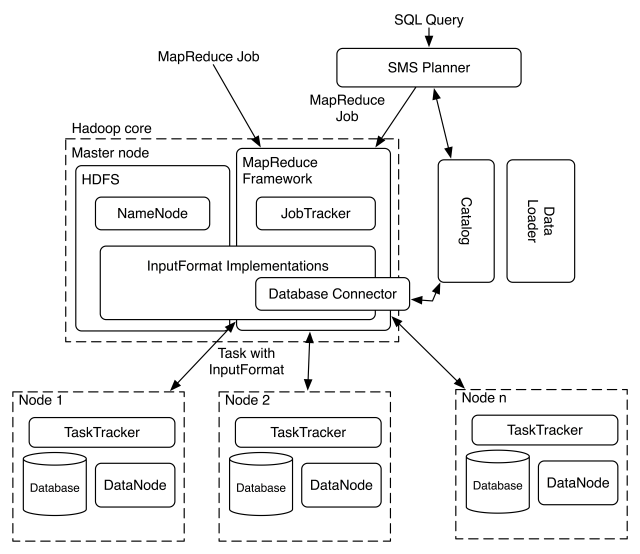
\includegraphics[width=0.7\textwidth]{images/hadoopdb-arch.png}
  \caption{The Architecture of HadoopDB\cite{journals/pvldb/AbouzeidBARS09}}
  \label{fig:hadoopdbarch}
\end{figure}

\section{Benchmarks}
The HadoopDB paper uses the same benchmarks as used in Stonebrakers comparison paper. These are
\begin{itemize}
\item Grep Task: \verb+SELECT * FROM Data WHERE field LIKE '%XYZ%';+
\item Selection Task: 

\verb+ SELECT pageUrl, pageRank FROM Rankings WHERE pageRank > 10;+
\item Aggregation Task
  \begin{enumerate}
  \item Smaller query:
\begin{verbatim}
SELECT SUBSTR(sourceIP, 1, 7), SUM(adRevenue) FROM UserVisits 
GROUP BY SUBSTR(sourceIP, 1, 7);
\end{verbatim}

  \item Larger query:
\begin{verbatim}
SELECT sourceIP, SUM(adRevenue) FROM UserVisits 
GROUP BY sourceIP;
\end{verbatim}

  \end{enumerate}
  \item Join Task:
\begin{verbatim}
SELECT sourceIP, COUNT(pageRank), SUM(pageRank),
SUM(adRevenue) FROM Rankings AS R, UserVisits AS UV
WHERE R.pageURL = UV.destURL AND
UV.visitDate BETWEEN '2000-01-15' AND '2000-01-22'
GROUP BY UV.sourceIP;
\end{verbatim}
  \item
\end{itemize}


Im Selection Task ist HadoopDB langsamer als Hadoop, widerspruch zwischen Diagramm und Text!




Lack of impact of HadoopDB:
  - Resonanz in Entwicklerkreisen:

    - Suche "HadoopDB" auf PostgreSQL Listenarchiv (8.4.2011): 4 Erwähnung seit einem Jahr, 15 total
      \url{http://search.postgresql.org/search?m=1}

    - Google Suche (7.4.): <10 unabhängige Erwähnungen, sonst nur Kopien der Presseerklärung und Präsentationen der Autoren

    - 22 Commits auf Sourceforge SVN (7.4.2011)

Commercialization as Hadapt

\subsection{Drawbacks of relational schemes}
  - Sparse vs. dense data

  - Entity-attribute-value model als Reaktion auf unflexibles relationales Model

  - Vergleich HBase/Cassandra mit Column Stores
    \url{http://dbmsmusings.blogspot.com/2010/03/distinguishing-two-major-types-of_29.html}

    - sparse (reference by row name)/dense(reference by position in column)
    - optimization: read-write/read
    - columns / column families
    - column names in HBase/Cassandra are often also data, since the scheme is not predefined

  - HBase 
    \url{http://twitter.com/#!/Hadapt/status/52357968141885441}
    28.3.2011 Storing data in our storage layer is 600 times faster than storing it in HBase for analysis. So we certainly don't use HBase!

- Wie gut reagieren RDBMSs auf scheme evolution?

\subsection{Practical evaluation}

Zu kompliziert:
\url{http://hadoopdb.sourceforge.net/guide} :
"a careful analysis of data and expected queries results in a significant performance boost at the expense of a longer loading. Two important things to consider are data partitioning and DB tuning (e.g. creating indices). Again, details of those techniques are covered in textbooks. For some queries, hash-partitioning and clustered indices improve HadoopDB's performance 10 times"

Two complicate systems to administrate: Hadoop+PostgreSQL

  - Storage waste:
    load data into HDFS, copy in local file system, load into postgreSQL

- access could not be granted to everybody. MapReduce allows to run add hock queries without scheme adaption and indices.

- Scheme / No scheme = Waterfal / Scrum, MR analyzes raw data


\section{Hive}

- Vorteil SQL: Beschreibt was, nicht wie. Optimierung wird der Software überlassen.
\section{Pig, Cascading, Sawzall}

\section{Conclusion}



% http://liinwww.ira.uka.de/bibliography/index.html
% http://de.wikipedia.org/wiki/BibTeX#Bibliographiedatenbanken
\bibliography{references}{}
\bibliographystyle{alphadin}
\end{document}

% LocalWords:  RDBMSs HadoopDB CPUs Stonebrakers nosqlsummer Stonebraker Abadi
% LocalWords:  Vertica Jagl Cloudbase Gartner streamy et al
